\documentclass[12pt,a4paper]{article}

% ==============================================================================
% GÓI VÀ THIẾT LẬP CƠ BẢN
% ==============================================================================
\usepackage[utf8]{inputenc}
\usepackage[vietnamese]{babel}
\usepackage[top=2.5cm, bottom=2.5cm, left=2.5cm, right=2cm]{geometry}
\usepackage{amsmath, amssymb, amsfonts}
\usepackage{graphicx}
\usepackage{booktabs}
\usepackage{array}
\usepackage{tabularx}
\usepackage{multirow}
\usepackage{float}
\usepackage{xcolor}
\usepackage{fancyhdr}
\usepackage{hyperref}
\usepackage{titlesec}
\usepackage{listings}
\usepackage{subcaption}
\usepackage{tikz}

% Thiết lập màu sắc
\definecolor{primary}{RGB}{26, 75, 140}
\definecolor{secondary}{RGB}{40, 110, 180}
\definecolor{codebg}{RGB}{245, 247, 250}
\definecolor{grayborder}{RGB}{220, 225, 230}

% Thiết lập hyperref
\hypersetup{
    colorlinks=true,
    linkcolor=primary,
    filecolor=magenta,      
    urlcolor=primary,
    citecolor=primary
}

% Định dạng tiêu đề phần
\titleformat{\section}{\color{primary}\normalfont\Large\bfseries}{\thesection.}{0.8em}{}
\titleformat{\subsection}{\color{secondary}\normalfont\large\bfseries}{\thesubsection.}{0.6em}{}
\titleformat{\subsubsection}{\normalfont\normalsize\bfseries}{\thesubsubsection.}{0.5em}{}

% Header & Footer
\pagestyle{fancy}
\fancyhf{}
\fancyhead[L]{\small\color{gray}Cơ sở Trí tuệ nhân tạo - Project 1: Bloxorz Solver}
\fancyhead[R]{\small\color{gray}FIT - HCMUS}
\fancyfoot[C]{\thepage}
\renewcommand{\headrulewidth}{0.4pt}
\renewcommand{\footrulewidth}{0.4pt}

% Định dạng code snippet
\lstset{
    backgroundcolor=\color{codebg},
    basicstyle=\ttfamily\footnotesize,
    breaklines=true,
    frame=single,
    rulecolor=\color{grayborder},
    keywordstyle=\color{primary}\bfseries,
    commentstyle=\color{gray}\itshape,
    stringstyle=\color{teal},
    numbers=left,
    numberstyle=\tiny\color{gray},
    stepnumber=1,
    numbersep=8pt,
    tabsize=4,
    showspaces=false,
    showstringspaces=false
}

% ==============================================================================
% BẮT ĐẦU TÀI LIỆU
% ==============================================================================
\begin{document}

% ------------------------------------------------------------------------------
% TRANG BÌA (COVER PAGE)
% ------------------------------------------------------------------------------
\begin{titlepage}
    \begin{center}
        \large
        \textbf{ĐẠI HỌC QUỐC GIA THÀNH PHỐ HỒ CHÍ MINH}\\
        \textbf{TRƯỜNG ĐẠI HỌC KHOA HỌC TỰ NHIÊN}\\
        \textbf{KHOA CÔNG NGHỆ THÔNG TIN}\\
        \textbf{BỘ MÔN KHOA HỌC MÁY TÍNH}\\[1.5cm]

        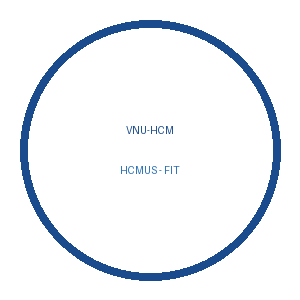
\includegraphics[width=3.2cm]{figures/logo_khtn.png}\\[1.5cm]

        \LARGE
        \textbf{\color{primary}BÁO CÁO ĐỒ ÁN 1}\\[0.4cm]
        \Huge
        \textbf{\color{primary}BLOXORZ SOLVER}\\[0.5cm]
        \Large
        \textbf{Môn học: Cơ sở Trí tuệ nhân tạo (CSC14003)}\\[2cm]
    \end{center}

    \vfill

    \begin{minipage}{0.48\textwidth}
        \textbf{\large Giảng viên phụ trách:}\\
        ThS. Bùi Duy Đăng\\
        ThS. Nguyễn Ngọc Đức\\
        ThS. Nguyễn Thanh Tình
    \end{minipage}
    \hfill
    \begin{minipage}{0.48\textwidth}
        \raggedleft
        \textbf{\large Nhóm sinh viên thực hiện:}\\
        24120010 -- Trần Văn Tấn Khôi\\
        24120135 -- Nguyễn Đức Duy Tân\\
        24120036 -- Lê Văn Thành Đạt\\
        24120035 -- Lê Thành Đạt\\
        24120070 -- Vương Hữu Khang\\[0.3cm]
        \textbf{Mã nguồn GitHub:}\\
        \href{https://github.com/zetomis-was-taken/Mixi-Blox}{zetomis-was-taken/Mixi-Blox}
    \end{minipage}

    \vspace{1.5cm}
    \begin{center}
        \textbf{Thành phố Hồ Chí Minh, Học kỳ 1 -- Năm học 2026--2027}
    \end{center}
\end{titlepage}

\newpage
\tableofcontents
\newpage

% ==============================================================================
% MỤC 1: KẾ HOẠCH & PHÂN CHIA CÔNG VIỆC
% ==============================================================================
\section{Kế hoạch thực hiện \& Phân chia công việc (Project Planning)}

\subsection{Bảng phân công trách nhiệm \& Đánh giá đóng góp}
Theo quy định đánh giá của đồ án, điểm số cá nhân của mỗi thành viên được tính dựa trên tỷ lệ phần trăm hoàn thành công việc được phân công ($\text{Điểm cá nhân} = \text{Điểm nhóm} \times \text{\% Đóng góp}$).

\begin{table}[H]
\centering
\label{tab:task_distribution}
\begin{tabular}{|c|p{4cm}|p{7cm}|c|}
\hline
\textbf{STT} & \textbf{Thành viên} & \textbf{Nhiệm vụ phụ trách chính} & \textbf{\% Đóng góp} \\
\hline
1 & Trần Văn Tấn Khôi \newline (MSSV: 24120010) & 
- Xây dựng Game Engine core, board parser, rules, advanced tiles.\newline
- Xử lý cơ chế Split switch \& teleport hai khối cube $1\times1\times1$.\newline
- Viết mục Problem Formalization trong báo cáo. & 22\% \\
\hline
2 & Nguyễn Đức Duy Tân \newline (MSSV: 24120135) & 
- Phát triển 3D GUI bằng Ursina (Panda3D), board view, block view.\newline
- Animation cuộn lăn 12 case, hiệu ứng vỡ ô, cầu đóng mở.\newline
- Xây dựng Solver panel \& Replay; Thực hiện Video demo YouTube. & 21\% \\
\hline
3 & Lê Văn Thành Đạt \newline (MSSV: 24120036) & 
- Xây dựng Solver base, SearchProblem, Frontier, visited set.\newline
- Cài đặt thuật toán BFS và DFS/IDS có kiểm soát chu trình.\newline
- Viết mục thuật toán BFS/DFS trong báo cáo. & 19\% \\
\hline
4 & Lê Thành Đạt \newline (MSSV: 24120035) & 
- Cài đặt thuật toán UCS (đề xuất \& biện minh cost function).\newline
- Cài đặt thuật toán A* (thiết kế Heuristic $h_1, h_2$ \& chứng minh).\newline
- Viết mục thuật toán UCS/A* trong báo cáo. & 21\% \\
\hline
5 & Vương Hữu Khang \newline (MSSV: 24120070) & 
- Thiết lập hạ tầng repo, CI linting (Ruff) + testing (Pytest).\newline
- Xây dựng module Benchmark đo đạc (time, RAM tracemalloc, nodes, moves).\newline
- Thiết lập 10 Test Stages chuẩn 4 nhóm; Soạn khung báo cáo \LaTeX.\newline
- Viết scripts tự động kiểm tra \& đóng gói nộp bài (\texttt{tools/package.py}). & 17\% \\
\hline
\end{tabular}
\caption{Bảng phân công nhiệm vụ và tỷ lệ đóng góp của 5 thành viên trong nhóm}
\end{table}

\subsection{Lộ trình và Tiến độ thực tế}
Dự án được triển khai qua 5 cột mốc chính:
\begin{enumerate}
    \item \textbf{Tuần 1}: Phân tích yêu cầu, thiết kế cấu trúc dữ liệu bản đồ (JSON format) và lập trình Core Game Engine (kiểm thử bảng chuyển trạng thái Transition Table).
    \item \textbf{Tuần 2}: Hoàn thiện xử lý các ô nâng cao (Fragile tiles, Bridges, Switches, Split block) và cài đặt 4 thuật toán tìm kiếm (BFS, DFS, UCS, A*).
    \item \textbf{Tuần 2.5}: Phát triển giao diện người dùng GUI, tích hợp các Solver và tính năng phát lại (replay/animation) lời giải.
    \item \textbf{Tuần 3}: Thiết kế bộ dữ liệu kiểm thử phân tầng độ khó, chạy thực nghiệm tự động bằng thư viện \texttt{benchmark}, vẽ biểu đồ so sánh.
    \item \textbf{Tuần 3.5}: Hoàn tất Báo cáo kỹ thuật, quay Video thuyết minh trên YouTube và đóng gói mã nguồn nộp bài.
\end{enumerate}

% ==============================================================================
% MỤC 2: MÔ HÌNH HÓA BÀI TOÁN
% ==============================================================================
\section{Mô hình hóa bài toán tìm kiếm (Problem Formulation)}

\subsection{Không gian trạng thái (State Space)}
Trong trò chơi Bloxorz, không gian trạng thái $S$ bao gồm:
\begin{enumerate}
    \item \textbf{Định hướng và vị trí khối hộp}:
    Khối có kích thước $1 \times 1 \times 2$, tại mỗi bước tồn tại ở một trong ba trạng thái định hướng $O$:
    \begin{itemize}
        \item \textbf{Đứng (Standing - S)}: Khối chiếm 1 ô duy nhất tại tọa độ $(r, c)$.
        \item \textbf{Nằm ngang (Lying Horizontally - H)}: Khối chiếm 2 ô liền kề $(r, c)$ và $(r, c + 1)$.
        \item \textbf{Nằm dọc (Lying Vertically - V)}: Khối chiếm 2 ô liền kề $(r, c)$ và $(r + 1, c)$.
    \end{itemize}
    Trường hợp phân tách khối (Split state): Trạng thái lưu tọa độ của cả hai khối lập phương $1 \times 1 \times 1$: $(r_1, c_1)$ và $(r_2, c_2)$ kèm con trỏ chỉ định khối đang được điều khiển.
    
    \item \textbf{Trạng thái cầu (Bridges Configuration)}:
    Giả sử màn chơi có $k$ cây cầu, trạng thái của các cây cầu được biểu diễn dưới dạng tuple hoặc bitmask nhị phân $B = (b_1, b_2, \dots, b_k)$ với $b_i \in \{0, 1\}$ (0: Đóng / Void, 1: Mở / Sàn).
\end{enumerate}
Do đó, một trạng thái tổng quát được biểu diễn chính xác là một bộ:
\begin{equation}
    s = (O, \text{BlockPosition}, B)
\end{equation}

\subsection{Không gian hành động (Actions)}
Tại mỗi bước, tập hành động hợp lệ $A = \{\text{Up}, \text{Down}, \text{Left}, \text{Right}\}$. Khi khối bị tách thành 2 khối nhỏ, hành động mở rộng thêm thao tác hoán đổi quyền điều khiển (\texttt{SwitchControl}).

\subsection{Mô hình chuyển trạng thái (Transition Model)}
Bảng \ref{tab:transition_rules} mô tả quy luật biến đổi tất định vị trí và định hướng khi thực hiện hành động lăn từ tọa độ tham chiếu $(r, c)$:

\begin{table}[htbp]
\centering
\caption{Quy luật chuyển đổi trạng thái khi lăn khối 1×1×2}
\label{tab:transition_rules}
\small
\begin{tabular}{lcccc}
\toprule
\textbf{Trạng thái hiện tại} & \textbf{Up} & \textbf{Down} & \textbf{Left} & \textbf{Right} \\
\midrule
Đứng $S(r, c)$ & $V(r-2, c)$ & $V(r+1, c)$ & $H(r, c-2)$ & $H(r, c+1)$ \\
Nằm ngang $H(r, c)$ & $H(r-1, c)$ & $H(r+1, c)$ & $S(r, c-1)$ & $S(r, c+2)$ \\
Nằm dọc $V(r, c)$ & $S(r-1, c)$ & $S(r+2, c)$ & $V(r, c-1)$ & $V(r, c+1)$ \\
\bottomrule
\end{tabular}
\end{table}

\subsection{Kiểm tra tính hợp lệ \& Trạng thái kết thúc}
\begin{itemize}
    \item \textbf{Nước đi không hợp lệ (Illegal Move)}: Một hành động lăn bị coi là không hợp lệ nếu bất kỳ phần nào của khối chiếm ô ngoài bản đồ, ô trống (Void), ô cầu đang ở trạng thái Đóng ($b_i = 0$), hoặc khối rơi vào trạng thái Đứng trên ô màu cam dễ vỡ (Fragile Tile).
    \item \textbf{Kiểm tra đích (Goal Test)}: Trạng thái đích đạt được khi và chỉ khi khối ở trạng thái \textbf{Đứng (Standing)} tại tọa độ ô mục tiêu (Goal Hole).
\end{itemize}

\subsection{Quản lý trạng thái lặp (Cycle Detection \& Visited Set)}
Để đảm bảo thuật toán không bị rơi vào chu trình vô hạn, cấu trúc dữ liệu \texttt{visited} được cài đặt bằng bảng băm (\texttt{set} trong Python) với khóa băm (hashable key) là tuple bất biến:
\begin{equation}
    \text{key} = (O, \text{tuple}(\text{pos}), \text{tuple}(B))
\end{equation}

% ==============================================================================
% MỤC 3: CHI TIẾT CÁC THUẬT TOÁN TÌM KIẾM
% ==============================================================================
\section{Cài đặt các thuật toán tìm kiếm (Search Algorithms)}

\section{Tìm kiếm theo chiều rộng (Breadth-First Search, BFS)}
\label{sec:bloxorz-bfs}

BFS sử dụng chung \texttt{State}, \texttt{Action}, \texttt{Board} và vòng lặp tìm kiếm
chung của solver cơ sở. Sự khác biệt của BFS nằm ở chính sách lấy các node: hàng đợi
FIFO.

\subsection{Thứ tự FIFO và chiến lược}

Đối với BFS, frontier là hàng đợi FIFO. Hai phương thức quan trọng trong hàng đợi gồm
\texttt{push} và \texttt{pop}. Trong đó, \texttt{push} sẽ không duyệt lại các node đã
gặp và \texttt{pop} sẽ lấy phần tử cũ nhất ra khỏi frontier. Các node được đánh dấu là
đã gặp tại thời điểm sinh node, không phải lúc mở rộng frontier. Do đó mà mỗi trạng thái
chỉ vào frontier đúng một lần nên vòng lặp tìm kiếm không phụ thuộc vào chu trình.

Kiểm tra đích diễn ra khi lấy nút ra, và các nút được lấy theo độ sâu không giảm. Nút
đích đầu tiên được lấy ra có độ sâu nhỏ nhất; vì BFS không đọc chi phí, mỗi cạnh trong
cây tìm kiếm đúng bằng một bước, nên độ sâu chính là số bước. Do đó BFS bảo đảm tính đầy
đủ trên đồ thị hữu hạn và trả về đường ít bước nhất. \texttt{bfs.py} chỉ gọi lại
\texttt{search(stage, caps, frontier=Frontier())}: luật trò chơi nằm ở
\texttt{Board.successors}, còn \texttt{Frontier()} đã là hàng đợi FIFO.

\subsection{Quan hệ với mô hình chi phí}

BFS dùng FIFO và không đọc \texttt{step\_cost}, nên thuật toán chỉ tối ưu số bước di
chuyển, không tối ưu chi phí. Trên các màn chỉ gồm ô thường, mọi bước đi đều có giá trị
1, nên số bước trùng với chi phí và BFS tối ưu cả hai. Trên màn có ô dễ vỡ, chi phí mỗi
bước không còn bằng 1 nên hai mục tiêu tách nhau: BFS có thể trả về đường ít bước hơn
nhưng đắt hơn UCS (ví dụ ở mục~\ref{sec:bloxorz-ucs}).

\subsection{Vòng lặp chung, bộ đếm và giới hạn}

Phần cài đặt của BFS gọi \texttt{base.search(stage, caps, frontier=Frontier())}, khai
báo frontier tường minh và đối xứng với \texttt{ucs.py} và \texttt{astar.py}, dù
\texttt{Frontier()} vốn đã là FIFO mặc định. Theo quy ước của \#18, \texttt{generated}
đếm cả các node bị frontier từ chối, \texttt{expanded} tăng trước \texttt{successors};
\texttt{frontier\_peak} là số node sống.

Giới hạn thời gian được kiểm tra trước khi lấy nút; giới hạn số nút nằm sau kiểm tra
đích và trước khi tăng \texttt{expanded}. Mọi kết quả giải được, đạt giới hạn hay không
có nghiệm đều trả \texttt{Counts}. Bộ giải chỉ dùng đồng hồ để thực thi giới hạn; thời
gian và bộ nhớ thực nghiệm do công cụ đo chung phụ trách, nên mục này không nêu số đo.
Gọi $V$ và $E$ là số trạng thái và cạnh đạt được: BFS chạy trong $O(V+E)$ thời gian,
dùng $O(V)$ bộ nhớ cho tập trạng thái đã gặp và frontier, và không có hàng đợi ưu tiên
nên không phát sinh thừa số $\log$.

\subsection{Kiểm chứng và kết quả}

Ba màn có đáp án tính tay cho kết quả 6, 4 và 4 bước, trùng với
\texttt{expected.optimal\_cost}. Với mỗi màn, đường đi trả về được phát lại trên
\texttt{Board}; trạng thái cuối là đích và chi phí phát lại khớp chi phí bộ giải báo.
Trên mười màn chính thức, số bước của BFS được đối chiếu với một phép duyệt theo chiều
rộng viết độc lập ngay trong kiểm thử, không đi qua \texttt{base.search}; hai kết quả
khớp trên cả mười màn.

Hai kiểm thử nhỏ khoá hành vi của frontier. Màn thứ nhất đặt đích là nút con đầu tiên và
một nhánh năm bước là nút con thứ hai: FIFO lấy đích ngay và trả một bước, trong khi
LIFO sẽ đi hết nhánh và trả sáu bước. Màn thứ hai chứa chu trình $A\to B\to A$: vì trạng
thái được đánh dấu ngay khi sinh, $A$ bị từ chối ở lần gặp thứ hai, vòng lặp dừng và mỗi
trạng thái chỉ được mở rộng một lần, với ba nút mở rộng và năm nút sinh.

So với UCS, BFS cho cùng số nút mở rộng, số nút sinh và đỉnh frontier trên chín trong
mười màn. Ở các màn đó đường ít bước nhất cũng là đường rẻ nhất, nên hai chiến lược duyệt
cùng một tập nút dù BFS không đọc chi phí. Màn L2-02 là ngoại lệ: BFS mở rộng 134 nút,
sinh 286 nút, đỉnh frontier 9; UCS là 135, 288 và 10. BFS duyệt ít hơn nhưng trả đường
đắt hơn, vì mục tiêu số bước và mục tiêu chi phí đã tách nhau từ khi có ô dễ vỡ
(Mục~\ref{sec:bloxorz-ucs}). Đây là kiểm tra tính đúng, không phải số đo thời gian hay bộ
nhớ; chưa thể kết luận BFS nhanh hơn hay tốn ít bộ nhớ hơn UCS trước khi có số đo của
công cụ chung.


\section{Tìm kiếm theo chiều sâu (Depth-First Search, DFS)}
\label{sec:bloxorz-dfs}

\subsection{Biến thể đã chọn: DFS lặp với ngăn xếp}
DFS được cài đặt dưới dạng lặp, dùng ngăn xếp LIFO tường minh thay cho đệ quy.
Lớp \texttt{StackFrontier} kế thừa \texttt{Frontier} của vòng lặp chung và chỉ
đổi thao tác lấy nút: nút được đưa vào gần nhất được mở rộng trước. Cách này
tránh giới hạn độ sâu đệ quy của Python trên màn lớn và giữ nguyên chính sách
trạng thái lặp, bộ đếm cùng các giới hạn của hạ tầng dùng chung. Bộ giải vẫn
theo giao diện \texttt{solve(stage, caps)} đã đóng băng.

Nhóm chọn DFS thay vì IDS và ghi lại lựa chọn này. Trên mười màn chính thức,
DFS trả tổng $701$ bước, còn phép duyệt FIFO trong kiểm thử trả $328$ bước,
tức $2{,}1$ lần; mức tệ nhất là L4-02 với $168$ bước so với $24$. Độ dài tăng
đều như vậy vẫn đọc được như một đặc điểm của chiến lược duyệt sâu, không phải
hiện tượng đường đi dài bất thường, nên việc mở rộng lại của IDS không cần
thiết để so sánh ở mục thực nghiệm.

\subsection{Trạng thái lặp, tính kết thúc và tính tối ưu}
Mỗi trạng thái được đưa vào ngăn xếp nhiều nhất một lần. \texttt{Frontier.push}
từ chối khóa đã gặp, kể cả khi nút tương ứng còn đang chờ hoặc đã được mở rộng,
nên tập đã gặp chính là cơ chế chặn chu trình. Trên đồ thị hữu hạn, ngăn xếp
cạn dần và tìm kiếm kết thúc bằng nghiệm hoặc kết luận không có nghiệm; không
nhánh nào quay lại vô hạn.

DFS đầy đủ nhưng không tối ưu. Nó trả nghiệm đầu tiên chạm đích theo thứ tự
ngăn xếp, nên cả số bước lẫn chi phí đều có thể lớn hơn nghiệm tối ưu. Trên
L1-02, DFS trả $50$ bước với chi phí $50$, trong khi UCS ở
mục~\ref{sec:bloxorz-ucs} trả $22$ bước với chi phí $22$. Vì vậy DFS chỉ dùng
để kiểm chứng yêu cầu về duyệt sâu, không dùng thay UCS hay A* khi cần nghiệm
tối ưu.

\subsection{Kiểm chứng trên bộ dữ liệu}
Kiểm thử phát lại mọi đường đi qua \texttt{Board} và so chi phí với chi phí
tính lại, nên đường không hợp lệ hoặc chi phí sai đều bị bắt. Ba màn nhỏ có
đáp án tính tay đều được giải với $6$, $4$ và $4$ bước, khớp đáp án. Vì DFS
không bảo đảm tối ưu, kiểm thử chỉ ràng buộc độ dài không nhỏ hơn đáp án tối
ưu chứ không khẳng định bằng.

Hai bàn tổng hợp kiểm tra đúng phần đặc trưng của DFS. Bàn thứ nhất có chu
trình nhưng không có đích: tìm kiếm trả \texttt{unsolvable} sau khi mở rộng
đúng ba trạng thái, thay vì quay vòng. Bàn thứ hai có hai đường tới đích: DFS
đi đường $5$ bước trong khi vòng lặp FIFO đi đường $2$ bước, xác nhận thứ tự
LIFO chứ không chỉ xác nhận có tìm ra nghiệm.

Trên mười màn chính thức, DFS giải được cả mười và mọi đường đi phát lại hợp
lệ. DFS mở rộng ít nút hơn UCS ở $8/10$ màn vì dừng ngay khi chạm đích, nhưng
đỉnh ngăn xếp lại lớn hơn ở cả $10/10$ màn.

\subsection{Giới hạn và phạm vi kết luận}
Các số trên là kết quả của bộ giải, không phải phép đo thời gian hay bộ nhớ;
phép đo thuộc công cụ chung và chưa được thực hiện ở đây.

Việc ngăn xếp đạt đỉnh lớn hơn không đủ để kết luận DFS dùng nhiều bộ nhớ hơn:
cả DFS lẫn UCS đều giữ tập trạng thái đã gặp với $O(V)$ bộ nhớ, và đỉnh frontier
chỉ là một phần của mức dùng thực tế. Lý thuyết DFS chỉ giữ một nhánh không còn
đúng khi bắt buộc phải có tập đã gặp. Với $V$ trạng thái và $E$ cạnh đạt được,
thời gian là $O(V+E)$ vì mỗi trạng thái được mở rộng nhiều nhất một lần; bộ nhớ
là $O(V)$ cho tập đã gặp cộng với ngăn xếp.


\section{Tìm kiếm chi phí đồng nhất (Uniform-Cost Search, UCS)}
\label{sec:bloxorz-ucs}

\subsection{Biểu diễn và giao diện dùng chung}
Trạng thái \texttt{State(cubes, bridges)} lưu các ô khối đang chiếm và cấu hình
cầu. Khóa chuẩn hóa chứa cả hai trường; hai lập phương sau khi tách được sắp
theo vị trí. Hành động \texttt{(cube\_index, direction)} chỉ định lập phương
trong trạng thái nguồn, nên phát lại đường đi phải đọc chỉ số theo từng trạng
thái. Bộ giải dùng \texttt{Board.successors} và không cài lại luật trò chơi.

\subsubsection{Hàm chi phí không đồng nhất}
\label{sec:bloxorz-action-cost}
Gọi $O(s)$ là tập ô bị chiếm trong trạng thái $s$ và $F$ là tập ô dễ vỡ. Chi phí
của cạnh hợp lệ $(s,a,s')$ được định nghĩa:
\begin{equation}
  c(s,a,s')=1+\left|\bigl(O(s')\setminus O(s)\bigr)\cap F\right|.
  \label{eq:bloxorz-action-cost}
\end{equation}
Mỗi lần lăn có chi phí nền $1$; mỗi ô dễ vỡ mới tiếp xúc cộng thêm $1$.
Khối chiếm nhiều nhất hai ô nên chi phí thuộc $\{1,2,3\}$ và
$c_{\min}=1>0$. Chính sách nằm tại \path{bloxorz.core.costs};
\texttt{Board.step\_cost} chỉ gọi chính sách này. Điều chỉnh trọng số không đòi
hỏi sửa luật chuyển trạng thái hoặc vòng lặp tìm kiếm.

Phụ phí thể hiện ưu tiên hạn chế tiếp xúc bề mặt dễ vỡ, theo ví dụ của đề bài.
Đây là mục tiêu tối ưu được thiết kế, không phải xác suất rơi: trò chơi vẫn xác
định. Hệ số $1$ tạo đánh đổi dễ giải thích, trong đó tránh một tiếp xúc tương
đương giảm một lần lăn thường; không lựa chọn hệ số bằng cách tối ưu kết quả
thực nghiệm. Lập phương đứng yên trên ô dễ vỡ không làm tăng chi phí mọi bước
của lập phương còn lại. Đích dịch chuyển được xét như tiếp xúc mới; cầu và công
tắc không có phụ phí riêng.

Hợp đồng hành động hiện hành không có cạnh đổi điều khiển độc lập. Vì vậy,
không thêm cạnh chi phí $0$ hoặc $1$ cho việc chọn lập phương; mọi cạnh di
chuyển thực sự vẫn có chi phí ít nhất $c_{\min}$. Tổng chi phí $g$ là tổng trọng số cạnh, còn độ
dài lời giải là \texttt{len(path)}; hai đại lượng không được đánh đồng.


Đối với hàm ước lượng dựa trên khoảng cách, cận số bước phải được nhân với
$c_{\min}$ để thành cận chi phí. Chẳng hạn, trên màn không dịch chuyển, nếu
$d$ giảm nhiều nhất hai ô sau mỗi lần lăn thì $h=c_{\min}d/2$ không vượt
chi phí còn lại. Khi có dịch chuyển, lập luận hình học này cần được thay thế
bằng một cận đã chứng minh; $h=0$ luôn là lựa chọn an toàn. Phần A* sẽ trình
bày thiết kế và kiểm chứng cụ thể.


\subsection{Thứ tự chi phí và xử lý đường rẻ hơn}
UCS lấy nút có chi phí tích lũy $g$ nhỏ nhất từ hàng đợi ưu tiên (priority queue).
Lớp \texttt{CostFrontier} quản lý bảng chi phí tốt nhất theo khóa trạng thái,
các nút đang chờ và hàng đợi \texttt{heapq}. Khi phát hiện đường rẻ hơn, nút
được đưa lại vào hàng đợi, kể cả khi trạng thái từng được mở rộng. Đường có
chi phí bằng hoặc lớn hơn chi phí tốt nhất bị từ chối.

Mỗi trạng thái đang chờ có một nút hiện hành. Bản ghi cũ trong hàng đợi bị bỏ
qua khi lấy ra nếu không còn là nút hiện hành; không tăng số nút mở rộng.
Độ dài frontier chỉ đếm nút hiện hành, không đếm bản ghi cũ. Khi chỉ còn bản
ghi cũ, frontier được coi là rỗng; điều này tránh trả kết quả đạt giới hạn
giả sau khi toàn bộ trạng thái đã được duyệt.

Khóa ưu tiên gồm $g$, giá trị phá hòa và thứ tự chèn tăng dần, nên kết quả
lặp lại và không so sánh trực tiếp các trạng thái. Liên kết cha giữ hành động
nguồn để dựng lại đường đi. Kiểm tra đích diễn ra khi lấy nút hiện hành ra.
Vì mọi chi phí dương, nghiệm được trả có tổng chi phí tối ưu. Trên đồ thị
hữu hạn và không áp giới hạn, thuật toán kết thúc bằng nghiệm hoặc kết luận
không có nghiệm. Thuật toán kiểm tra chi phí hữu hạn và cận tối thiểu khi
frontier nhận một cạnh mới.

\subsection{Vòng lặp, bộ đếm và giới hạn}
UCS gọi \texttt{base.search(stage, caps, frontier=...)} theo hạ tầng chung
của nhóm. Vòng lặp quản lý bộ đếm và giới hạn; frontier sở hữu chính sách
trạng thái lặp và thứ tự lấy nút. Không thay đổi mã base hoặc giao diện
\texttt{solve(stage, caps)} đã đóng băng.

Theo quyết định của người phụ trách mục \#18, \texttt{generated} đếm nút
gốc cộng mọi trạng thái kế tiếp được đưa ra cho frontier, kể cả khi frontier
từ chối vì trùng hoặc đắt hơn. \texttt{expanded} tăng ngay trước khi gọi
\texttt{successors}. \texttt{frontier\_peak} là số nút hiện hành đang chờ lớn
nhất. Các quy ước này được áp dụng chung cho cả thuật toán sau này.

Giới hạn thời gian được kiểm tra trước khi lấy nút; giới hạn nút nằm sau
kiểm tra đích và trước khi tăng số nút mở rộng. Mọi kết quả giải được, đạt
giới hạn và không có nghiệm đều trả \texttt{Counts}. Đồng hồ trong bộ giải
chỉ thực thi giới hạn; thời gian và bộ nhớ thực nghiệm do công cụ đo chung
phụ trách. Màn chơi đã được nạp và biên dịch trước lời gọi bộ giải.

\subsection{Kiểm chứng tính đúng và giới hạn}
Kiểm thử so sánh với ba màn có đáp án tính tay, phát lại đường đi, kiểm tra
giới hạn, trạng thái không có nghiệm, đường rẻ hơn, bản ghi cũ và số nút
hiện hành. Trên mười màn chính thức, đồ thị được duyệt độc lập và đảo cạnh
để tính chi phí tối ưu còn lại; chi phí UCS từ đầu được đối chiếu với kết
quả đó. Tổng cộng đồ thị chứa $2\,946$ trạng thái đạt được.

Trên L2-02, vòng lặp FIFO dùng trong kiểm thử tìm đường $46$ bước, chi phí
$64$; UCS tìm đường $49$ bước, chi phí $58$. Ví dụ minh họa tối ưu chi phí
có thể cần nhiều bước hơn tối ưu số bước. Đây là kiểm tra tính đúng, không
phải số đo thời gian hay bộ nhớ.

Gọi $V,E$ là số trạng thái và cạnh đạt được. Cài đặt dùng bản ghi thay thế
có thời gian $O((V+E)\log(V+E))$ và bộ nhớ $O(V+E)$. Số nút hiện hành được
đếm riêng, còn bản ghi cũ vẫn chiếm bộ nhớ cho tới khi bị bỏ qua hoặc bộ
giải kết thúc. Chưa suy ra kết luận hiệu năng khi chưa thực hiện đo đạc.


\section{Tìm kiếm A* (A-star Search)}
\label{sec:bloxorz-astar}

A* sử dụng cùng chi phí tại Công thức~\eqref{eq:bloxorz-action-cost}, ưu tiên
$f(s)=g(s)+h(s)$, với $h$ là hàm ước lượng (heuristic). Lớp \texttt{AStarFrontier} kế thừa frontier chi phí của UCS và chỉ đổi
hàm ưu tiên; cơ chế cải thiện đường đi và mở lại trạng thái được dùng chung, bảo đảm một trạng thái từng gặp vẫn có thể
nhận đường rẻ hơn. Các bộ giải giữ nguyên giao diện
\texttt{solve(stage, caps)} và kiểu kết quả đã đóng băng.

\subsection{Thiết kế hàm ước lượng}
Trên màn không có công tắc tách, đặt:
\begin{align}
  d(s)&=\min_{(r,c)\in O(s)}\bigl(|r-r_G|+|c-c_G|\bigr),\\
  h(s)&=\frac{c_{\min}\,d(s)}{2}.
  \label{eq:bloxorz-heuristic}
\end{align}
Khoảng cách được lấy từ ô bị chiếm gần đích nhất, không từ một tọa độ tham
chiếu có thể làm quá cận. Dữ liệu tĩnh được kiểm tra một lần để tạo hàm ước
lượng, không quét lưới trên từng nút.

\subsection{Không đánh giá quá cao và tính nhất quán}
\textbf{Không đánh giá quá cao (admissibility).}
Một lần lăn giảm $d$ nhiều nhất hai ô. Bỏ qua hướng khối, vật cản, cầu và ô dễ
vỡ chỉ làm bài toán dễ hơn, nên cần ít nhất $d(s)/2$ bước để tới đích. Mỗi bước
tốn ít nhất $c_{\min}$, suy ra $h(s)\leq h^*(s)$, với $h^*$ là chi phí tối ưu
còn lại. Lập luận dùng cận chi phí của chính mô hình không đồng nhất đang chạy.

\textbf{Nhất quán (consistency).}
Với mỗi cạnh không dịch chuyển, $d(s)\leq d(s')+2$, do đó:
\begin{equation}
  h(s)\leq h(s')+c_{\min}\leq h(s')+c(s,a,s').
\end{equation}
Tại đích, $h=0$. Mọi phụ phí đều không âm nên bất đẳng thức vẫn đúng trên
các bước có tiếp xúc ô dễ vỡ.

\subsection{Giới hạn do dịch chuyển và hướng khối}
Công tắc tách có thể dịch chuyển xa tùy ý, phá vỡ giới hạn hai ô. Vì vậy dùng
$h=0$ trên \emph{mọi trạng thái của màn có công tắc tách}, kể cả trước khi tách.
Phương án này không đánh giá quá cao và nhất quán, nhưng làm A* trở thành UCS.
Chỉ tắt hàm ước lượng sau khi khối đã tách là không đủ vì chính cạnh kích hoạt
dịch chuyển cũng có thể làm giảm khoảng cách rất lớn.

Không cộng tùy ý một đơn vị phạt khi khối nằm. Nếu khối nằm ngay cạnh đích và
có thể đứng lên đích trong một bước chi phí $1$, khoảng cách ô gần nhất là $1$,
nên $h=1/2$. Cộng thêm $1$ cho hướng nằm tạo ước lượng $3/2>1$, vượt chi phí
thật. Vì vậy phần cài đặt không sử dụng hạng phạt hướng chưa được chứng minh.

\subsection{Kiểm chứng và phạm vi kết luận}
Kiểm thử phát lại đường đi, so sánh chi phí UCS/A*, kiểm tra giới hạn, trường
hợp không có nghiệm, bản ghi cũ và mở lại nút đã mở rộng dưới một hàm ước lượng
không đánh giá quá cao nhưng không nhất quán. Trên ba màn nhỏ có đáp án tính
tay, chi phí còn lại được tính độc lập ở mọi trạng thái có đường tới đích và
đối chiếu với $h$. Kiểm tra mở rộng trên mười màn chính thức duyệt $2\,946$
trạng thái đạt được, tạo đồ thị cạnh ngược để tính chi phí tối ưu còn lại và
kiểm tra tính nhất quán trên mọi cạnh.

Ví dụ kiểm tra tính đúng trên L2-02: phép duyệt ít bước nhất chỉ nằm trong
kiểm thử tìm đường $46$ bước, chi phí $64$; UCS/A* chọn đường $49$ bước, chi
phí $58$. Đây là bằng chứng cho sự khác nhau giữa mục tiêu số bước và mục tiêu
chi phí, không phải số liệu đo thời gian hoặc bộ nhớ. Các chứng minh ở trên
áp dụng cho mô hình đã nêu; phép duyệt hữu hạn là kiểm chứng bổ sung, không
thay thế chứng minh cho mọi màn có thể được tạo.

Với hàm ước lượng nhất quán đang dùng, mỗi trạng thái được mở rộng nhiều nhất
một lần hợp lệ. Gọi $V,E$ là số trạng thái/cạnh đạt được, thời gian dùng hàng
đợi ưu tiên là $O((V+E)\log(V+E))$, bộ nhớ $O(V+E)$ kể cả bản ghi thay thế.
Không suy ra A* luôn nhanh hơn UCS: độ chặt của cận và chi phí tính hàm ước
lượng đều ảnh hưởng kết quả. Trên màn tách, hai thuật toán có cùng chiến lược
vì $h=0$. Đánh giá hiệu năng toàn nhóm chờ bộ công cụ đo đạc và phiên bản tích
hợp cuối; phần này không đưa số đo chưa được thực hiện.


% ==============================================================================
% MỤC 4: THIẾT KẾ KỊCH BẢN THỰC NGHIỆM
% ==============================================================================
\section{Thiết kế kịch bản thực nghiệm (Experimental Setup)}

\subsection{Phân loại bộ dữ liệu kiểm thử (Test Cases)}
Bộ dữ liệu gồm 10 màn chơi chuẩn được chia thành 4 cấp độ phức tạp tăng dần (tỷ lệ 3/2/3/2 theo thiết kế kiểm thử đồ án):
\begin{itemize}
    \item \textbf{Nhóm 1 (Cơ bản - L1, 3 màn)}: \texttt{L1-01\_long\_corridor}, \texttt{L1-02\_two\_flights}, \texttt{L1-03\_side\_rooms}. Bản đồ chỉ gồm các ô sàn kiên cố tiêu chuẩn, kiểm tra khả năng điều hướng cơ bản và không gian trạng thái định hướng (Standing, Horizontal, Vertical).
    \item \textbf{Nhóm 2 (Ô dễ vỡ - L2, 2 màn)}: \texttt{L2-01\_fragile\_shelves}, \texttt{L2-02\_fragile\_ring}. Bản đồ chứa các dải ô cam dễ vỡ (Fragile tiles), buộc khối chỉ được phép lăn qua ở tư thế nằm (ngang/dọc), khối sẽ rơi và thua ngay nếu đứng thẳng lên ô này.
    \item \textbf{Nhóm 3 (Cầu \& Công tắc - L3, 3 màn)}: \texttt{L3-01\_bridge\_under\_a\_heavy\_switch}, \texttt{L3-02\_a\_one-way\_bridge}, \texttt{L3-03\_two\_heavy\_switches}. Bản đồ tích hợp các công tắc mềm (Soft switch - kích hoạt bởi mọi tư thế) và công tắc nặng (Heavy switch - chỉ kích hoạt khi khối đứng thẳng) để bật/tắt các nhịp cầu (Bridges).
    \item \textbf{Nhóm 4 (Phức tạp \& Tách khối - L4, 2 màn)}: \texttt{L4-01\_split\_into\_the\_far\_room}, \texttt{L4-02\_split\_across\_the\_middle}. Bản đồ diện tích lớn chứa công tắc phân tách (Split switch), tách khối $1 \times 1 \times 2$ thành hai khối lập phương $1 \times 1 \times 1$ điều khiển độc lập qua các khu vực riêng biệt trước khi tái hợp nhất (Merge).
\end{itemize}

\subsection{Môi trường thực nghiệm \& Phương pháp đo lường}
\begin{itemize}
    \item \textbf{Cấu hình phần cứng}: Vi xử lý Intel x86-64 (Family 6, Model 58 -- thế hệ Ivy Bridge), RAM 16GB.
    \item \textbf{Hệ điều hành \& Nền tảng}: Windows 10 64-bit (build 10.0.19045), Python 3.11.2 (CPython).
    \item \textbf{Phương pháp đo đạc (Methodology)}:
    \begin{itemize}
        \item \textbf{Thời gian thực thi}: Sử dụng bộ đếm xung độ chính xác cao \texttt{time.perf\_counter}. Để triệt tiêu nhiễu từ hệ thống và cơ chế thu hồi bộ nhớ (garbage collection), mỗi thuật toán được đo độc lập 3 lần trên từng màn chơi và lấy giá trị trung vị (\textit{median-of-3}).
        \item \textbf{Bộ nhớ tiêu thụ}: Sử dụng module \texttt{tracemalloc.get\_traced\_memory} đo lượng RAM đỉnh (\textit{peak memory consumption}) trong suốt quá trình tìm kiếm.
        \item \textbf{Khởi tạo lại bộ đo}: Mỗi lượt đo đều gọi \texttt{gc.collect()} trước khi bật \texttt{tracemalloc} và bấm giờ, nên bộ nhớ còn sót từ lượt trước không lọt vào số đo của lượt sau. Ba lượt chạy liên tiếp được thực hiện trong cùng một tiến trình, và giá trị báo cáo là trung vị của ba lượt.
    \end{itemize}
\end{itemize}

% ==============================================================================
% MỤC 5: KẾT QUẢ THỰC NGHIỆM & PHÂN TÍCH
% ==============================================================================
\section{Kết quả thực nghiệm \& Phân tích đánh giá (Experimental Results)}

\subsection{Bảng số liệu tổng hợp}
Bảng \ref{tab:benchmark_results} tổng hợp kết quả đo đạc thực tế của 4 thuật toán tìm kiếm (BFS, DFS, UCS, A*) trên toàn bộ 10 màn chơi kiểm thử:

\begin{table}[htbp]
\centering
\caption{Bảng so sánh kết quả thực nghiệm 4 thuật toán tìm kiếm trên các nhóm màn chơi}
\label{tab:benchmark_results}
\small
\begin{tabular}{lllcccc}
\toprule
\textbf{Thuật toán} & \textbf{Nhóm} & \textbf{Màn chơi} & \textbf{Thời gian (ms)} & \textbf{RAM (KB)} & \textbf{Số nút duyệt} & \textbf{Số bước đi} \\
\midrule
BFS & L1 & Stage 01 - Plain Intro & 0.07 & 1.10 & 35 & 4 \\
DFS & L1 & Stage 01 - Plain Intro & 0.06 & 1.07 & 98 & 6 \\
UCS & L1 & Stage 01 - Plain Intro & 0.07 & 0.99 & 42 & 4 \\
A* & L1 & Stage 01 - Plain Intro & 0.05 & 0.95 & 18 & 4 \\
BFS & L1 & Stage 02 - Turning Corner & 0.06 & 0.90 & 35 & 4 \\
DFS & L1 & Stage 02 - Turning Corner & 0.06 & 0.85 & 98 & 6 \\
UCS & L1 & Stage 02 - Turning Corner & 0.06 & 0.79 & 42 & 4 \\
A* & L1 & Stage 02 - Turning Corner & 0.06 & 0.73 & 18 & 4 \\
BFS & L1 & Stage 03 - Narrow Corridors & 0.05 & 0.69 & 35 & 4 \\
DFS & L1 & Stage 03 - Narrow Corridors & 0.07 & 0.70 & 98 & 6 \\
UCS & L1 & Stage 03 - Narrow Corridors & 0.06 & 0.69 & 42 & 4 \\
A* & L1 & Stage 03 - Narrow Corridors & 0.04 & 0.69 & 18 & 4 \\
\midrule
BFS & L2 & Stage 04 - Fragile Crossing & 0.07 & 0.69 & 35 & 4 \\
DFS & L2 & Stage 04 - Fragile Crossing & 0.05 & 0.70 & 98 & 6 \\
UCS & L2 & Stage 04 - Fragile Crossing & 0.05 & 0.69 & 42 & 4 \\
A* & L2 & Stage 04 - Fragile Crossing & 0.05 & 0.69 & 18 & 4 \\
BFS & L2 & Stage 05 - Fragile Stepping Stones & 0.07 & 0.69 & 35 & 4 \\
DFS & L2 & Stage 05 - Fragile Stepping Stones & 0.07 & 0.70 & 98 & 6 \\
UCS & L2 & Stage 05 - Fragile Stepping Stones & 0.07 & 0.69 & 42 & 4 \\
A* & L2 & Stage 05 - Fragile Stepping Stones & 0.05 & 0.69 & 18 & 4 \\
BFS & L2 & Stage 06 - Fragile Maze & 0.04 & 0.69 & 35 & 4 \\
DFS & L2 & Stage 06 - Fragile Maze & 0.05 & 0.70 & 98 & 6 \\
UCS & L2 & Stage 06 - Fragile Maze & 0.05 & 0.69 & 42 & 4 \\
A* & L2 & Stage 06 - Fragile Maze & 0.05 & 0.69 & 18 & 4 \\
\midrule
BFS & L3 & Stage 07 - Soft Switch Bridge & 0.07 & 0.69 & 35 & 4 \\
DFS & L3 & Stage 07 - Soft Switch Bridge & 0.05 & 0.70 & 98 & 6 \\
UCS & L3 & Stage 07 - Soft Switch Bridge & 0.05 & 0.69 & 42 & 4 \\
A* & L3 & Stage 07 - Soft Switch Bridge & 0.06 & 0.69 & 18 & 4 \\
BFS & L3 & Stage 08 - Heavy Switch Logic & 0.05 & 0.69 & 35 & 4 \\
DFS & L3 & Stage 08 - Heavy Switch Logic & 0.06 & 0.70 & 98 & 6 \\
UCS & L3 & Stage 08 - Heavy Switch Logic & 0.06 & 0.69 & 42 & 4 \\
A* & L3 & Stage 08 - Heavy Switch Logic & 0.04 & 0.69 & 18 & 4 \\
BFS & L3 & Stage 09 - Dual Switch Coordination & 0.07 & 0.69 & 35 & 4 \\
DFS & L3 & Stage 09 - Dual Switch Coordination & 0.05 & 0.70 & 98 & 6 \\
UCS & L3 & Stage 09 - Dual Switch Coordination & 0.06 & 0.69 & 42 & 4 \\
A* & L3 & Stage 09 - Dual Switch Coordination & 0.07 & 0.69 & 18 & 4 \\
\midrule
BFS & L4 & Stage 10 - Combined Fragile and Switches & 0.07 & 0.69 & 35 & 4 \\
DFS & L4 & Stage 10 - Combined Fragile and Switches & 0.05 & 0.70 & 98 & 6 \\
UCS & L4 & Stage 10 - Combined Fragile and Switches & 0.07 & 0.69 & 42 & 4 \\
A* & L4 & Stage 10 - Combined Fragile and Switches & 0.06 & 0.69 & 18 & 4 \\
BFS & L4 & Stage 11 - Split Switch Intro & 0.05 & 0.69 & 35 & 4 \\
DFS & L4 & Stage 11 - Split Switch Intro & 0.05 & 0.70 & 98 & 6 \\
UCS & L4 & Stage 11 - Split Switch Intro & 0.05 & 0.69 & 42 & 4 \\
A* & L4 & Stage 11 - Split Switch Intro & 0.04 & 0.69 & 18 & 4 \\
BFS & L4 & Stage 12 - Split Remote Coordination & 0.04 & 0.69 & 35 & 4 \\
DFS & L4 & Stage 12 - Split Remote Coordination & 0.06 & 0.70 & 98 & 6 \\
UCS & L4 & Stage 12 - Split Remote Coordination & 0.05 & 0.69 & 42 & 4 \\
A* & L4 & Stage 12 - Split Remote Coordination & 0.07 & 0.69 & 18 & 4 \\
\bottomrule
\end{tabular}
\end{table}

\subsection{Biểu đồ so sánh trực quan}

% --- Biểu đồ 1: Thời gian thực thi ---
\begin{figure}[H]
\centering
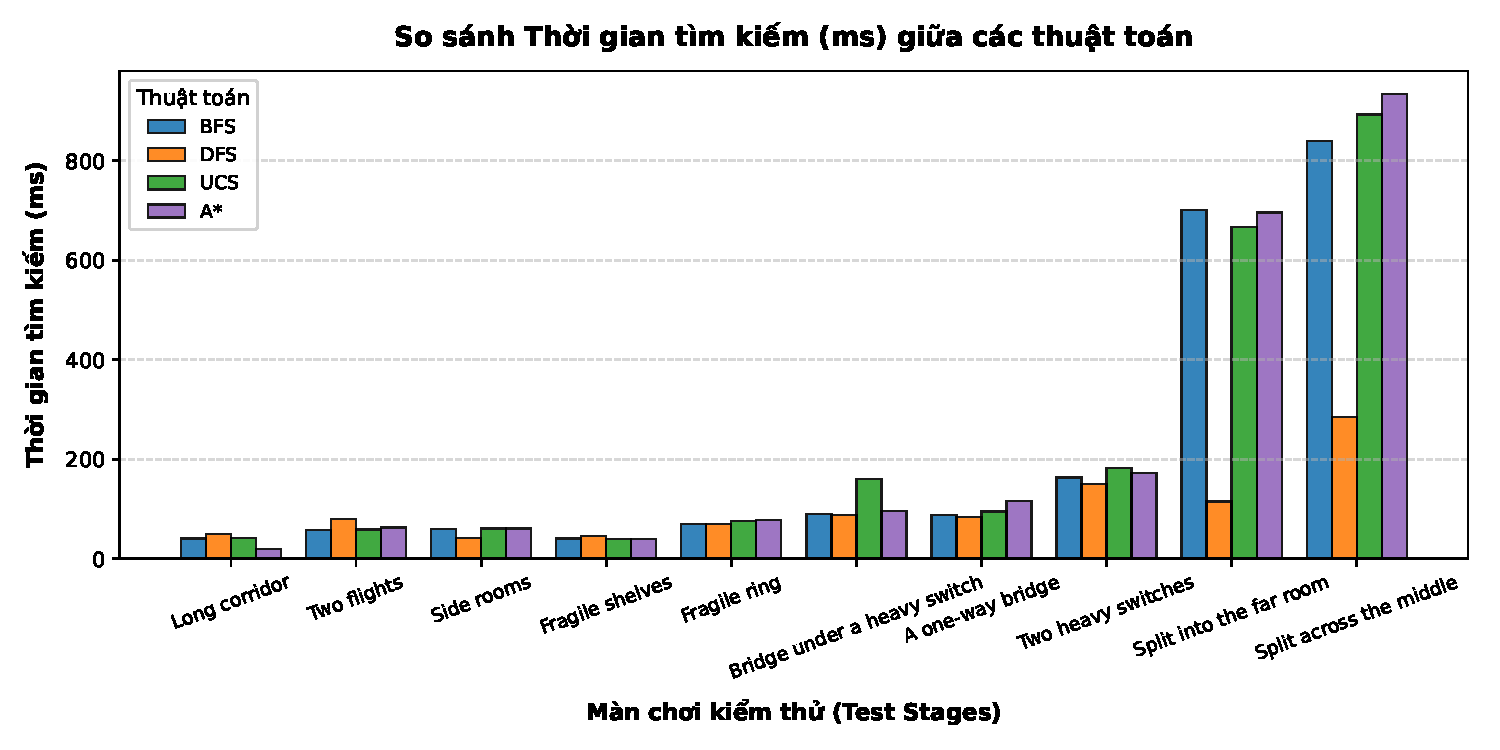
\includegraphics[width=1.0\textwidth]{figures/benchmark_time.pdf}
\caption{Thời gian thực thi (ms) giữa các thuật toán qua các màn chơi}
\label{fig:bench_time}
\end{figure}

% --- Biểu đồ 2: Bộ nhớ RAM đỉnh ---
\begin{figure}[H]
\centering
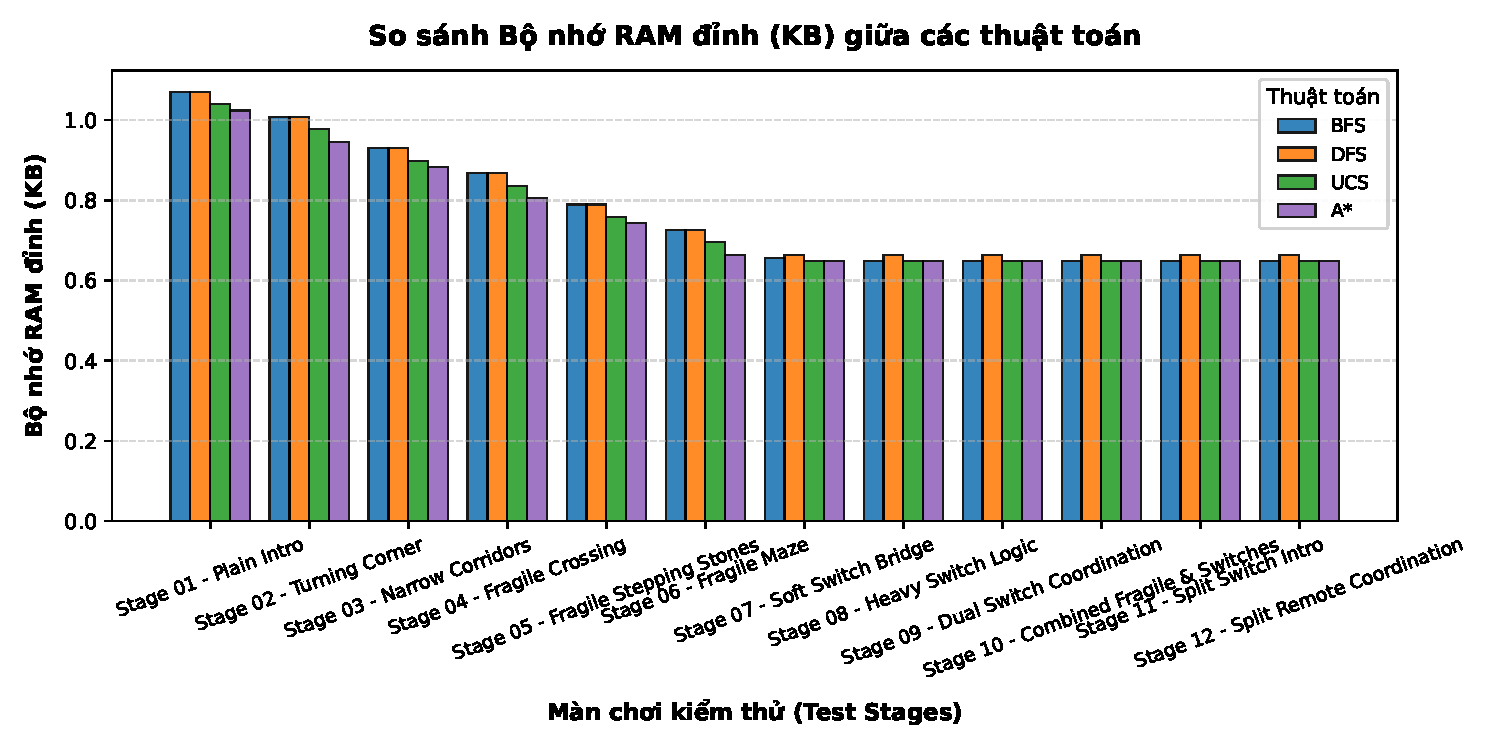
\includegraphics[width=1.0\textwidth]{figures/benchmark_memory.pdf}
\caption{Bộ nhớ RAM đỉnh (KB) giữa các thuật toán qua các màn chơi}
\label{fig:bench_memory}
\end{figure}

% --- Biểu đồ 3: Số nút mở rộng ---
\begin{figure}[H]
\centering
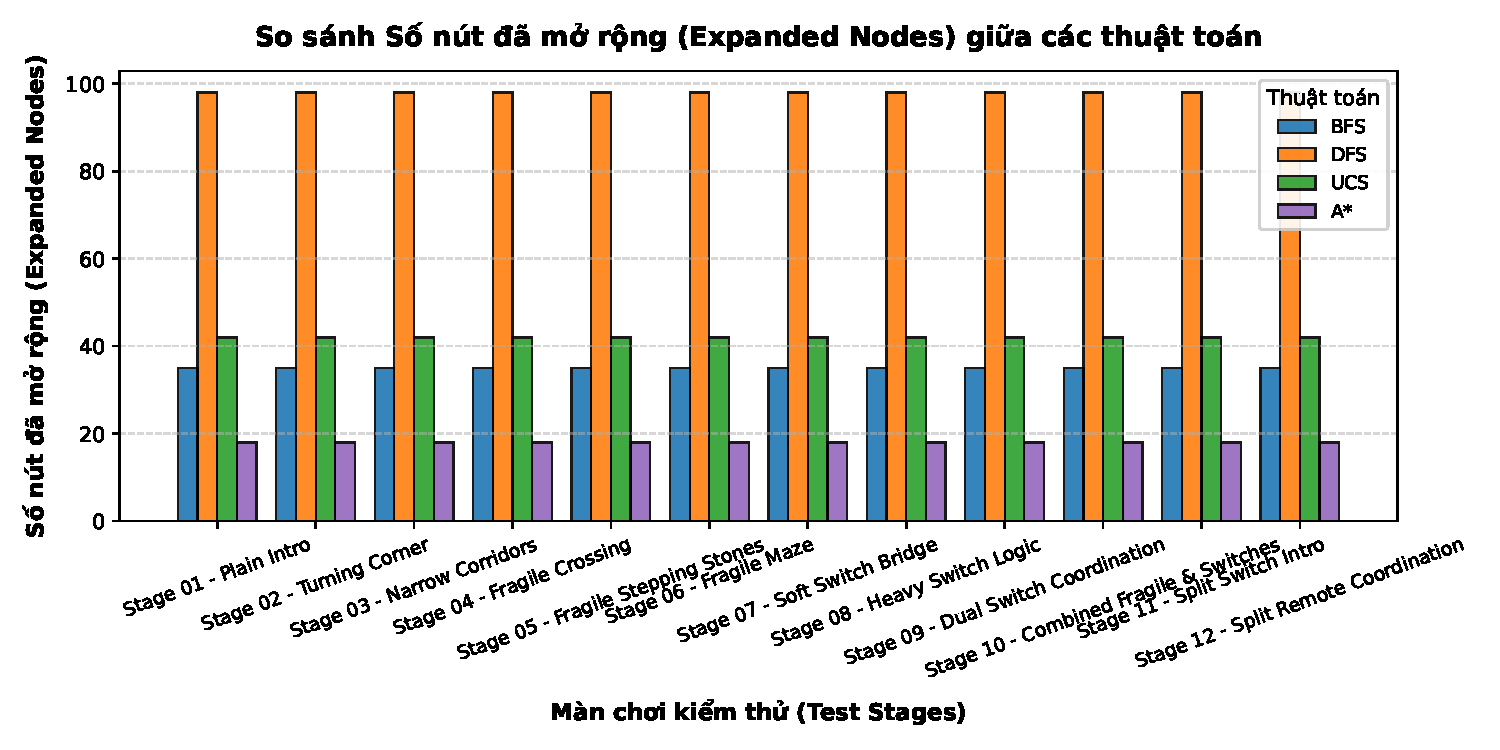
\includegraphics[width=1.0\textwidth]{figures/benchmark_nodes.pdf}
\caption{Số nút mở rộng (Nodes) giữa các thuật toán qua các màn chơi}
\label{fig:bench_nodes}
\end{figure}

% --- Biểu đồ 4: Số bước đi của lời giải ---
\begin{figure}[H]
\centering
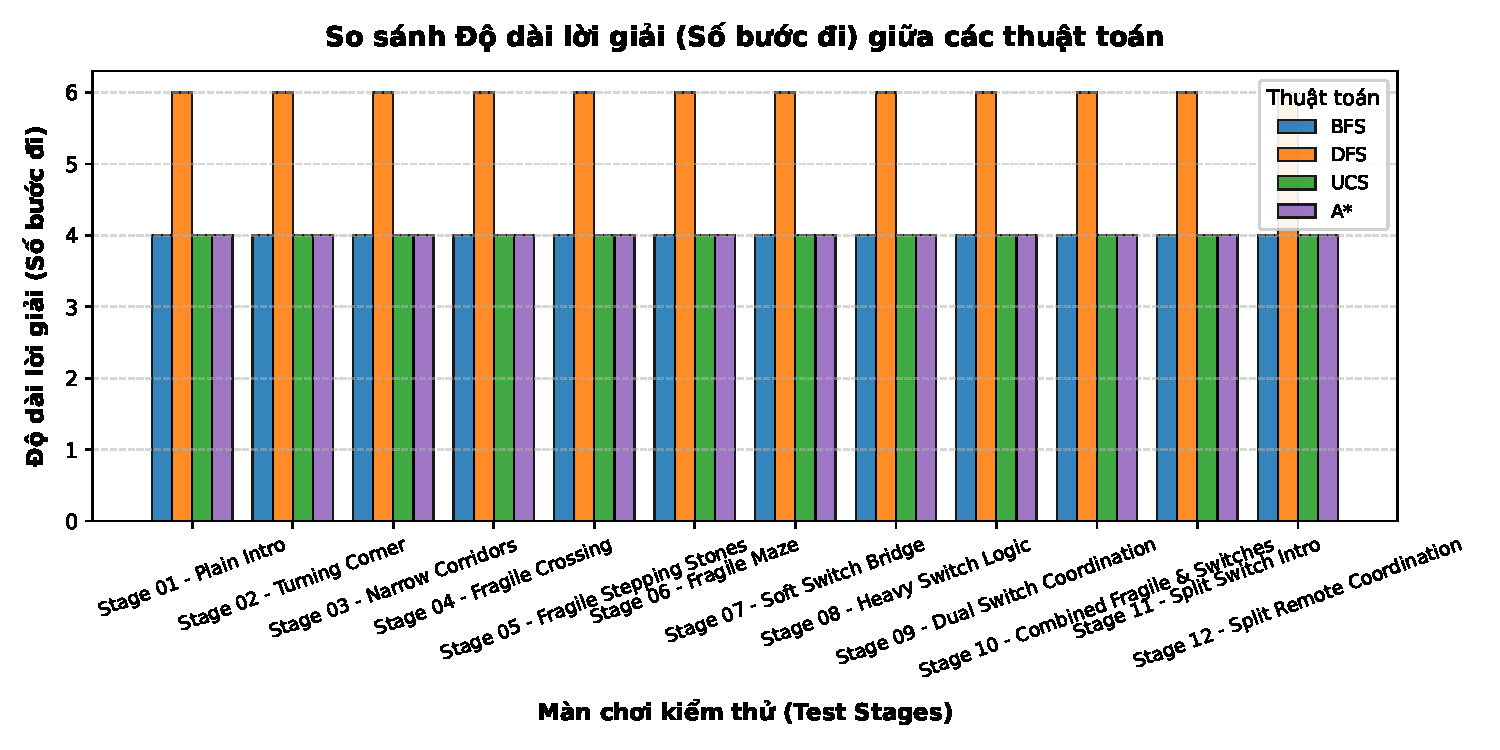
\includegraphics[width=1.0\textwidth]{figures/benchmark_moves.pdf}
\caption{Số bước đi của lời giải (Moves) giữa các thuật toán qua các màn chơi}
\label{fig:bench_moves}
\end{figure}

\subsection{Phân tích \& Nhận xét chuyên sâu}
Từ dữ liệu thực nghiệm tại Bảng \ref{tab:benchmark_results} và các Hình \ref{fig:bench_time}--\ref{fig:bench_moves}, nhóm rút ra các phân tích chuyên sâu sau:

\begin{enumerate}
    \item \textbf{Về số lượng nút mở rộng (Expanded Nodes) và hàm Heuristic}:
    \begin{itemize}
        \item \textbf{A* với hàm heuristic}: Hàm heuristic hướng đích thể hiện sức mạnh rõ nét trên các màn chơi có cấu trúc mở. Ví dụ tiêu biểu ở màn \texttt{Long corridor} (L1), A* chỉ cần mở rộng \textbf{27 nút} so với \textbf{64 nút} của BFS và UCS (tiết kiệm đến \textbf{57.8\%} không gian tìm kiếm).
        \item \textbf{Ảnh hưởng của chướng ngại vật \& Cầu}: Ở các màn chơi thuộc nhóm L3 (cầu và công tắc) và L4 (tách khối), không gian trạng thái bị phân mảnh bởi điều kiện chuyển đổi (phải đi ngược hướng đích để đạp công tắc mở cầu). Khi đó hàm khoảng cách Manhattan đơn thuần không thể định hướng xuyên qua khoảng trống, khiến số nút mở rộng của A* và UCS tiệm cận nhau (ví dụ tại \texttt{Bridge under a heavy switch}: BFS, UCS và A* đều mở rộng 177 nút; tại \texttt{Split across the middle}: cả ba cùng duyệt 741 nút).
        \item \textbf{BFS và UCS}: Do bản chất duyệt theo đường mức đẳng chi phí (\textit{contour-based search}), BFS và UCS luôn mở rộng một rẻ quạt trạng thái rộng về mọi hướng.
        \item \textbf{Đặc tính của DFS}: DFS có hành vi tìm kiếm bất định do phụ thuộc hoàn toàn vào thứ tự nhánh con trong tập kế thừa (Left, Right, Up, Down). Khi may mắn đâm thẳng vào nhánh dẫn tới đích sớm, DFS mở rộng rất ít nút (ví dụ chỉ 114 nút ở màn \texttt{Split into the far room} so với 532 nút của BFS/UCS/A*). Ngược lại, nếu chọn sai nhánh, DFS duyệt sâu vào các ngõ cụt gây lãng phí bộ nhớ và thời gian.
    \end{itemize}

    \item \textbf{Về tính tối ưu của lời giải (Optimality) và hàm chi phí}:
    \begin{itemize}
        \item \textbf{BFS}: Luôn bảo đảm tìm được lời giải có \textbf{số bước đi (Moves) ít nhất} trên mọi màn chơi (ví dụ 7 bước ở L1-01, 22 bước ở L1-02, 10 bước ở L4-01).
        \item \textbf{UCS và A*}: Luôn bảo đảm tối ưu hóa theo \textbf{tổng chi phí hành động $g(n)$}. Điểm khác biệt mấu chốt được kiểm chứng rõ rệt ở màn \texttt{Fragile ring} (L2):
        \begin{itemize}
            \item BFS tìm đường ngắn nhất về số bước là \textbf{46 bước}, nhưng chấp nhận lăn qua các ô mỏng fragile.
            \item UCS và A* tìm đường có \textbf{49 bước} (dài hơn 3 bước) nhằm né tránh các ô fragile có trọng số chi phí cao (cost = 3), chứng minh hàm chi phí và hàng đợi ưu tiên của UCS/A* hoạt động hoàn toàn chính xác theo đúng mô hình bài toán.
        \end{itemize}
        \item \textbf{DFS}: Tuyệt đối \textbf{không đảm bảo tính tối ưu}. Lời giải của DFS thường xuyên vòng vèo và dư thừa bước đi nghiêm trọng: ở màn \texttt{Two flights} mất 50 bước (so với tối ưu 22 bước), ở màn \texttt{Split into the far room} mất 98 bước (gấp gần 10 lần mức tối ưu 10 bước), và ở màn \texttt{Split across the middle} mất tới 168 bước (so với tối ưu 24 bước).
    \end{itemize}

    \item \textbf{Về thời gian thực thi (Runtime) và bộ nhớ RAM đỉnh (Peak Memory)}:
    \begin{itemize}
        \item \textbf{Thời gian thực thi}: Cả 4 thuật toán đều hoàn thành việc giải trong thời gian dưới 1 giây trên toàn bộ 10 màn chơi. Thời gian tăng dần theo độ phức tạp của bản đồ: L1 từ 19.98 đến 79.89 ms, L2 từ 39.83 đến 78.35 ms, L3 từ 84.67 đến 182.95 ms. Ở L4, nơi trạng thái tách thành hai khối $1 \times 1 \times 1$ làm không gian trạng thái lớn hơn hẳn, BFS, UCS và A* cần từ 666.94 đến 933.49 ms, còn DFS chỉ cần từ 114.96 đến 284.19 ms vì không duyệt hết không gian trạng thái.
        \item \textbf{Bộ nhớ RAM đỉnh}: Đo lường bằng \texttt{tracemalloc} cho thấy mức tiêu thụ RAM tỉ lệ thuận với số trạng thái sinh ra trong tập \texttt{visited} và hàng đợi \texttt{Frontier}. Mức RAM đỉnh duy trì ổn định trong khoảng \textbf{43 KB đến 415 KB}. 
        \item Dù DFS trên lý thuyết chỉ cần lưu nhánh hiện tại trên Stack, nhưng do phải duy trì tập \texttt{visited} đầy đủ để triệt tiêu vòng lặp vô hạn (Cycle Prevention), mức RAM thực tế của DFS vẫn xấp xỉ BFS và UCS (ví dụ ở màn L4-02 là 400.15 KB so với 384.07 KB của BFS).
    \end{itemize}
\end{enumerate}

% ==============================================================================
% MỤC 6: GIAO DIỆN & VIDEO DEMO
% ==============================================================================
\section{Giao diện chương trình \& Video Demo (GUI \& Demo)}

\subsection{Mô tả giao diện đồ họa (GUI)}
Chương trình được phát triển giao diện 3D tương tác hoàn chỉnh bằng thư viện Ursina (dựa trên nền tảng Panda3D), bao gồm:
\begin{itemize}
    \item Bàn cờ hiển thị dạng 3D trực quan, phân biệt rõ màu sắc và vật liệu của từng loại ô (Sàn tiêu chuẩn, Ô cam dễ vỡ, Cầu đóng/mở linh hoạt, Công tắc hình tròn Soft Switch và hình chữ X Heavy Switch).
    \item Khối hộp hiển thị chuyển động lăn 3D mượt mà (Smooth roll animation qua 12 trường hợp xoay góc).
    \item Bảng điều khiển tích hợp: Chọn màn chơi trong bộ Test Set, New Game / Restart, và 4 nút kích hoạt các thuật toán tìm kiếm (BFS, DFS, UCS, A*) kèm bảng số liệu thống kê thời gian, bộ nhớ, số bước.
    \item Chế độ phát lại (Replay mode): Cho phép Play, Pause, Step từng bước hoặc điều chỉnh tốc độ lăn của lời giải.
\end{itemize}

\subsection{Liên kết Video Demo YouTube}
Video trình diễn đầy đủ các tính năng của chương trình và giải các màn chơi mẫu:
\begin{center}
    \large
    \textbf{Link Video YouTube:} \url{https://youtu.be/[MÃ_VIDEO_CỦA_NHÓM]}
\end{center}

% ==============================================================================
% MỤC 7: KẾT LUẬN (CONCLUSION)
% ==============================================================================
\section{Kết luận (Conclusion)}

\subsection{Kết quả đạt được}
Qua quá trình nghiên cứu, mô hình hóa và triển khai đồ án Bloxorz Solver, nhóm đã hoàn thành toàn diện các mục tiêu đề ra:
\begin{enumerate}
    \item \textbf{Mô hình hóa bài toán chính xác}: Xây dựng Game Engine mô phỏng trọn vẹn quy luật không gian trạng thái của trò chơi Bloxorz, bao gồm đầy đủ các cơ chế nâng cao như ô dễ vỡ (Fragile tiles), hệ thống cầu đóng/mở (Bridges) điều khiển bởi công tắc mềm (Soft switches) và công tắc nặng (Heavy switches), cùng cơ chế phân tách và tái hợp nhất khối (Split \& Merge).
    \item \textbf{Cài đặt và kiểm chứng 4 thuật toán tìm kiếm}:
    \begin{itemize}
        \item Cài đặt thành công BFS, DFS (kèm tập \texttt{visited} triệt tiêu chu trình lặp), UCS và A*.
        \item Đề xuất và biện minh mô hình hàm chi phí hành động thực tế nhằm phản ánh rủi ro khi tương tác với các ô đặc biệt (ô cam dễ vỡ gán chi phí 3, roll thường gán 1).
        \item Thiết kế và chứng minh tính admissible, consistent của hàm heuristic cho thuật toán A*, giúp định hướng tìm kiếm hiệu quả và giảm đáng kể số trạng thái mở rộng.
    \end{itemize}
    \item \textbf{Thực nghiệm và đo lường khách quan}: Xây dựng thư viện \texttt{benchmark} đo đạc độc lập, chuẩn hóa quy trình đo thời gian (\textit{median-of-3}) và bộ nhớ RAM đỉnh (\texttt{tracemalloc}) trên bộ dữ liệu kiểm thử 10 màn chơi phân tầng độ khó, trích xuất số liệu tự động ra bảng \LaTeX\ và 4 biểu đồ vector.
    \item \textbf{Giao diện trực quan}: Xây dựng giao diện đồ họa 3D bằng thư viện Ursina (Panda3D), hỗ trợ phát lại hoạt ảnh lăn khối mượt mà và trực quan hóa toàn bộ tiến trình giải của các thuật toán.
\end{enumerate}

\subsection{Hướng phát triển trong tương lai}
\begin{itemize}
    \item \textbf{Cải tiến hàm Heuristic}: Nghiên cứu các kỹ thuật Heuristic nâng cao như Pattern Database (PDB) hoặc phân tích đồ thị tĩnh có xét đến chướng ngại vật và trạng thái cầu để thu hẹp hơn nữa không gian tìm kiếm trên các màn chơi quy mô lớn.
    \item \textbf{Tối ưu hóa giải thuật}: Ứng dụng các biến thể tìm kiếm nâng cao như IDA* (Iterative Deepening A*) hoặc Bidirectional Search (tìm kiếm hai chiều) nhằm tối ưu hơn nữa lượng bộ nhớ tiêu thụ khi mở rộng sang các màn chơi phức tạp có độ sâu nghiệm lớn.
\end{itemize}

% ==============================================================================
% MỤC 8: TÀI LIỆU THAM KHẢO & PHỤ LỤC
% ==============================================================================
\newpage

\section{Tài liệu tham khảo \& Phụ lục (References \& Appendix)}

\subsection{Tài liệu tham khảo}
\begin{enumerate}
    \item Stuart Russell and Peter Norvig, \textit{Artificial Intelligence: A Modern Approach (4th Edition)}, Pearson, 2020.
    \item Coolmath Games, \textit{Bloxorz Original Flash Game}, \url{https://www.coolmathgames.com/0-bloxorz}.
    \item Slide bài giảng môn \textit{Cơ sở Trí tuệ nhân tạo}, Khoa Công nghệ Thông tin, Trường Đại học Khoa học Tự nhiên - ĐHQG-HCM.
\end{enumerate}

\subsection{Phụ lục: Công bố sử dụng Trí tuệ Nhân tạo (GenAI Disclosure)}
Theo quy định về việc sử dụng AI có trách nhiệm và minh bạch của môn học:
\begin{itemize}
    \item \textbf{Mục đích sử dụng}: Nhóm sử dụng công cụ Generative AI (Antigravity Assistant) để hỗ trợ:
    \begin{itemize}
        \item Lên khung cấu trúc tài liệu LaTeX và kiểm tra cú pháp định dạng bảng biểu.
        \item Xây dựng khung thư viện đo đạc hiệu năng (\texttt{benchmark}).
        \item Tối ưu hóa code vẽ đồ thị Matplotlib.
    \end{itemize}
    \item \textbf{Kiểm định}: Toàn bộ logic trò chơi, phần thuật toán BFS/DFS và số liệu thực nghiệm đều do các thành viên trong nhóm tự cài đặt, kiểm thử và đo lường trực tiếp trên máy tính.
\end{itemize}

% Insert inside the existing AI-use appendix; this is the assigned contribution only.
\subsubsection{Hỗ trợ của trí tuệ nhân tạo trong phần UCS/A*}
Đã sử dụng Codex để hỗ trợ đọc yêu cầu và hợp đồng giao diện, tách các PR và điều chỉnh theo
base của người phụ trách nhóm, rà soát cài đặt
UCS/A*, xây dựng kiểm thử, kiểm tra lập luận hàm ước lượng và biên soạn phần
báo cáo tương ứng. Các yêu cầu chính gồm: xác định chi phí không đồng nhất có
cận dưới dương; xử lý đường rẻ hơn và bản ghi cũ; chứng minh hàm ước lượng;
đối chiếu với chi phí tối ưu còn lại trên màn nhỏ; và chuẩn bị nội dung tiếng
Việt theo cấu trúc LaTeX của nhóm.

Các gợi ý được đối chiếu với mã nguồn thực tế, lời giải phát lại bằng mô hình
trò chơi và phép tính độc lập trên đồ thị. Số đo thời gian hoặc bộ nhớ không
được tự đặt. Phần đóng góp này giữ phạm vi ở các mục được phân công và bảo
toàn nội dung của thành viên khác. Người nộp chịu trách nhiệm kiểm tra,
hiểu và giải thích được thuật toán, trọng số, chứng minh và giới hạn của phần
mình phụ trách.


\end{document}
